\documentclass[11pt,a4paper]{article}
\usepackage[margin=23mm,top=21mm,bottom=21mm]{geometry}
\usepackage{fontspec,kotex}
\setmainfont{Arial}
\setsansfont{Arial}
\setmonofont{Menlo}
\setmainhangulfont[ItalicFont={Apple SD Gothic Neo},ItalicFeatures={FakeSlant=.16}]{Apple SD Gothic Neo}
\setsanshangulfont[ItalicFont={Apple SD Gothic Neo},ItalicFeatures={FakeSlant=.16}]{Apple SD Gothic Neo}
\usepackage{amsmath,amssymb,booktabs,tabularx,array,longtable,multirow}
\usepackage[table]{xcolor}
\usepackage{tikz}
\usetikzlibrary{positioning,arrows.meta,shapes.geometric,calc}
\usepackage{enumitem,fancyhdr,titlesec,listings,xurl,hyperref}
\definecolor{ink}{HTML}{223746}
\definecolor{accent}{HTML}{315F7C}
\definecolor{pale}{HTML}{E8EFF4}
\definecolor{muted}{HTML}{596774}
\definecolor{linegray}{HTML}{C6D0D8}
\hypersetup{colorlinks=true,urlcolor=accent,linkcolor=accent,pdfauthor={KIT 프로젝트 팀},pdftitle={고객 행동 시뮬레이터 Feature와 데이터 설계 v4},pdfsubject={검색·CS 제외 6종 구성의 원천 학습과 시뮬레이터 계약}}
\pagestyle{fancy}\fancyhf{}
\fancyhead[L]{\footnotesize\color{muted}KIT\quad Keep In Touch}
\fancyhead[R]{\footnotesize\color{muted}설계 v4\quad |\quad 6종 이벤트 / KIT39 / raw5}
\fancyfoot[C]{\footnotesize\color{muted}KIT\quad |\quad \thepage}
\renewcommand{\headrulewidth}{0.25pt}
\setlength{\headheight}{14pt}
\setlength{\parindent}{0pt}\setlength{\parskip}{6pt}
\linespread{1.12}
\setlength{\emergencystretch}{3em}
\titleformat{\section}{\Large\bfseries\color{ink}}{\thesection}{.6em}{}
\titleformat{\subsection}{\normalsize\bfseries\color{ink}}{\thesubsection}{.6em}{}
\titlespacing*{\section}{0pt}{0pt}{11pt}
\titlespacing*{\subsection}{0pt}{9pt}{5pt}
\setlist[itemize]{leftmargin=1.4em,itemsep=3pt,topsep=3pt}
\setlist[enumerate]{leftmargin=1.5em,itemsep=3pt,topsep=3pt}
\newcolumntype{Y}{>{\raggedright\arraybackslash}X}
\newcolumntype{P}[1]{>{\raggedright\arraybackslash}p{#1}}
\renewcommand{\arraystretch}{1.24}
\setlength{\tabcolsep}{5pt}
\newcommand{\code}[1]{{\ttfamily\footnotesize\nolinkurl{#1}}}
\newcommand{\note}[1]{\par\noindent\colorbox{pale}{\parbox{\dimexpr\linewidth-2\fboxsep}{\small #1}}\par}
\newcommand{\page}{\clearpage}
\newcommand{\thead}{\rowcolor{pale}}
\lstset{basicstyle=\ttfamily\footnotesize,columns=fullflexible,keepspaces=true,breaklines=true,breakatwhitespace=false,frame=single,rulecolor=\color{linegray},backgroundcolor=\color{white},showstringspaces=false,xleftmargin=4pt,xrightmargin=4pt,aboveskip=7pt,belowskip=7pt}
\setcounter{tocdepth}{1}
\begin{document}
\thispagestyle{fancy}
{\Huge\bfseries\color{ink}고객 행동 시뮬레이터\par}
\vspace{5pt}
{\LARGE\color{ink}Feature와 데이터 설계\par}
\vspace{10pt}
{\Large 버전 4 수정판\par}
{\large 검색·CS를 제외한 6종 이벤트와 39개 Feature\par}
\vspace{9pt}
{\small KIT Keep In Touch\quad |\quad 2026년 11월 15일}

이 문서는 기존 설계의 업무 기록·시점·장바구니·쿠폰·구매 상품별 별점 계약을 정리한 \textbf{버전 4 수정판}이다. 사용자 지시에 따라 검색과 CS를 현재 생성·모델 준비·Feature·주간 출력에서 제외했다. 이벤트는 조회, 담기, 제거, 구매, 쿠폰 사용, 상품 별점 리뷰의 여섯 종류다.

재학습 범위도 이 6종 파이프라인이다. 쇼핑 결정은 Cosmetics의 네 관측 행동과 추론된 세션 종료로 IRL을 학습한다. 구매에 붙는 쿠폰 사용은 회계 이벤트이며, 별점 리뷰는 기존 Amazon/Olist 원천 적합 구성요소를 사용한다. 별도의 신규 리뷰 IRL 알고리즘이나 관측되지 않은 리뷰의 구매 인과효과를 추가하지 않는다.

\note{문서 버전 4, raw schema 5, 생성기 버전, Feature 버전은 서로 다른 식별자다. 이번 재학습 수치·실행 결과·기본 채택 판정은 뒤의 「이번 재학습과 실행 결과」가 기준이다. 이전 8종·45개 Feature 실행을 현재 성과로 바꾸어 부르지 않는다.}
\vspace{12pt}
\textbf{적용 범위}\quad 사용자 시뮬레이터, 원시 기록, 관측 Feature, 주간 실험 출력 및 재학습 근거. 하위 예측기나 새로운 리뷰 알고리즘을 추가하는 문서는 아니다.
\page
\renewcommand{\contentsname}{문서 안내}
\tableofcontents
\vspace{10pt}
\note{설계·이벤트·원시 기록, 원천 학습·잠재 성향·방문 시계, Feature 사전, 실험·검증 순서로 구성한다. 실제 재학습·생성 결과는 별도 결과 절에 제시한다. 각 수치의 원천·모형·시점을 함께 확인한다.}

\page
\section{현재 범위와 여섯 이벤트}
\begin{tabularx}{\linewidth}{@{}P{.19\linewidth}P{.24\linewidth}Y@{}}
\thead 이벤트 & 관측 의미 & 생성·연결 규칙\\\midrule
\code{view} & 상품 조회와 표시가격 & 같은 상품의 반복 조회도 기록. 수량은 NULL.\\[4pt]
\code{cart} & 장바구니 담기 & 상품 1개를 추가. 잔량은 다음 세션에도 유지.\\[4pt]
\code{remove_from_cart} & 장바구니 제거 & 실제 보유 상품 1개를 차감. 음수 재고 금지.\\[4pt]
\code{purchase} & 하나의 구매 결정 & Order 한 개와 다품목 OrderItem에 연결. 상품·수량은 Event가 아니라 주문상품에서 읽음.\\[4pt]
\code{coupon_usage} & 구매에 적용된 할인 & 실제 purchase에 같은 고객·세션·시각으로 연결. 최고 단가 구매품목 1개 할인.\\[4pt]
\code{review} & 구매 상품의 1--5점 별점 & 구매 $\times$ 서로 다른 상품마다 최대 한 번. 구매 후 비동기 도착.\\\bottomrule
\end{tabularx}

\subsection{이벤트와 상태의 구분}
진입기 ENTRY, 활동기 HOME, 이탈기 EXIT는 원시 세션에서 재구성하는 life-cycle 상태다. 별도 이벤트 종류가 아니다. 검색·CS는 이번 파이프라인에서 생성하지 않는다. 과거 raw4/5의 여덟 이벤트를 읽는 validator는 기존 자료의 재현을 위해 보존한다.

\subsection{계속 유지하는 요구}
업무 테이블은 7개, 기본 이탈은 4주·28일 미방문이다. 상품 가격·실제 결제액·세션 간 장바구니·고정 Treatment/Control·발송·사용·비용 로그를 유지한다. 리뷰 텍스트, 환불·취소·원가·배송비·세금은 현재 범위에 없다.

\subsection{현재 버전 식별}
\code{event_scope_version=shopping_coupon_review_v1}, \code{raw_schema_version=5}, 확장 Feature는 \code{kit39-review-cart-v2}다. 모델·엔진·설정 SHA와 dataset ID를 함께 확인한다. 같은 생성기 버전 문자열만으로 과거 8종과 현재 6종을 구별하지 않는다.

\page
\section{일곱 업무 관계와 원시 로그}
업무 기록에는 잠재 성향이나 미래 label을 넣지 않는다. 사용자별 실험 배정·결과·life-cycle·생성 진단은 별도 sidecar다.

\begin{center}
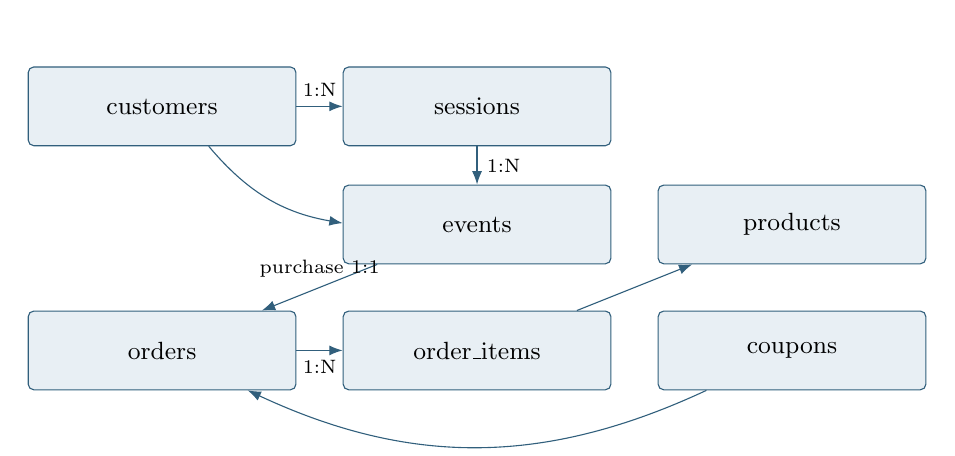
\begin{tikzpicture}[>=Latex,box/.style={draw=accent,fill=pale,rounded corners=2pt,align=center,font=\small,minimum width=34mm,minimum height=10mm},every edge/.style={draw=accent,->}]
\node[box] (c) at (-4,2.1) {customers};
\node[box] (s) at (0,2.1) {sessions};
\node[box] (e) at (0,.6) {events};
\node[box] (p) at (4,.6) {products};
\node[box] (o) at (-4,-1) {orders};
\node[box] (i) at (0,-1) {order\_items};
\node[box] (q) at (4,-1) {coupons};
\path (c) edge node[above,font=\scriptsize]{1:N} (s)
(s) edge node[right,font=\scriptsize]{1:N} (e)
(c) edge[bend right=20] (e)
(e) edge node[above,font=\scriptsize]{purchase 1:1} (o)
(o) edge node[below,font=\scriptsize]{1:N} (i)
(i) edge (p)
(q) edge[bend left=25] (o);
\end{tikzpicture}
\end{center}

{\small\begin{tabularx}{\linewidth}{@{}P{.19\linewidth}Y@{}}
\thead 관계 / 키 & 주요 필드와 참조\\\midrule
\code{customers} & \code{customer_id}, \code{signed_up_at}. persona는 고객 고정 업무 컬럼이 아님.\\
\code{products} & \code{product_id}, \code{category_id}, \code{unit_price_minor}.\\
\code{sessions} & \code{session_id}, 고객 FK, \code{started_at}, \code{ended_at}.\\
\code{events} & \code{event_id}, 고객·세션, 시각·종류, 상품·수량·표시가격, purchase/coupon/주문행 연결, 별점.\\
\code{orders} & \code{order_id}, 고유 \code{purchase_event_id}, \code{checkout_source}, 쿠폰, gross/discount/paid.\\
\code{order_items} & 복합키 \code{order_id,line_no}, 상품 FK, 수량, 구매단가.\\
\code{coupons} & \code{coupon_id}, 고객 FK, 발송·만료, 할인율, 정책, 발송비.\\\bottomrule
\end{tabularx}}

현재 Event는 canonical 17컬럼이다. 과거 호환용 \code{contact_id}는 현재 생성에서 NULL이며 CS 생성을 뜻하지 않는다. purchase의 품목은 OrderItem, review의 실제 구매는 \code{related_purchase_event_id}, 상품·주문행은 \code{product_id/order_line_no}로 확인한다.

\page
\section{가격·장바구니·주문 회계}
\subsection{가격과 단위}
Cosmetics의 실제 통화는 확인되지 않아 \code{SOURCE_UNSPECIFIED}다. 1 minor는 원천 가격 단위의 0.01이다. 원화를 뜻하지 않으며 임의 환산하지 않는다. 실행 카탈로그는 원천의 양수 관측 최빈가격을 상품별 고정단가로 사용한다. 행동 직전 표시단가와 실제 주문상품 단가를 로그로 남긴다.

\subsection{지속 장바구니}
고객 $u$, 상품 $p$의 cart는 엄격한 과거 로그를 시간·event ID 순서로 재생한다. 담기는 1개 추가하고 제거는 실제 보유분을 차감한다. 세션 종료나 조회 상품 변경으로 cart를 비우지 않는다.
\[
q_{u,p}^{+}=q_{u,p}^{-}+\text{담기량}-\text{제거량}-\text{이번 구매의 실제 보유 차감량},\qquad q_{u,p}^{+}\ge0.
\]
\begin{tabularx}{\linewidth}{@{}P{.18\linewidth}Y@{}}\thead 구매 경로 & cart 변화\\\midrule
\code{cart} & basket 전량이 실제 보유량 이내. 구매한 부분만 차감.\\
\code{buy_now} & 직접 구매. 기존 cart는 보존. 다품목도 허용.\\
\code{mixed} & 상품마다 $\min(\text{보유량},\text{구매량})$ 차감. 보유분과 직접 구매분이 모두 존재.\\\bottomrule\end{tabularx}

예를 들어 cart에 A 1개·B 1개가 있을 때 A 2개를 mixed 구매하면 A 1개만 차감하고 B는 남는다. 관측 시작 전 cart가 미상인 원천에서 임의의 초기 담기를 만들어 채우지 않는다. 생성 기록은 empty cart에서 시작하는 완전한 이력이다.

\subsection{한 번만 계산하는 결제}
\[
\mathrm{gross}=\sum_{l}q_l p_l,\qquad
\mathrm{paid}=\mathrm{gross}-\mathrm{discount}.
\]
모든 금액은 정수 minor다. 같은 주문의 Event·OrderItem·coupon usage를 각각 매출로 더하지 않는다. 소수 수량, 비유한 값, 음수 재고, FK 불일치와 회계 불일치는 저장 전에 거절한다.

\page
\section{진입기·활동기·이탈기와 관측 시점}
\subsection{원시 세션에서 계산하는 life-cycle}
\begin{center}
\begin{tikzpicture}[>=Latex,node distance=15mm,box/.style={draw=accent,fill=pale,rounded corners=2pt,minimum width=30mm,minimum height=11mm,font=\small}]
\node[box] (a) {ENTRY};\node[box,right=of a] (b) {HOME};\node[box,right=of b] (c) {EXIT};
\draw[->,accent] (a) -- node[above,font=\scriptsize]{첫 재방문} (b);
\draw[->,accent] (b) -- node[above,font=\scriptsize]{28일 미방문} (c);
\draw[->,accent] (c.south) to[bend left=25] node[below,font=\scriptsize]{관측된 귀환} (b.south);
\end{tikzpicture}
\end{center}
최초 관측 세션은 ENTRY, 첫 재방문부터 HOME, 마지막 세션 시작 이후 28일이 지나면 EXIT다. 최초 세션 뒤 재방문 없이 28일이 지나도 EXIT가 된다. 이탈 뒤 실제 귀환하면 HOME으로 돌아간다. 미래 방문을 미리 보고 과거 상태를 정하지 않는다. 정확히 28일 clock에서는 EXIT timer 뒤 HOME을 기록한다.

ENTRY는 실제 신규 가입, EXIT는 영구 탈퇴의 실측 정답이 아니다. 원천에 실제 가입일이 없어 생성 signup은 구조적 시계다. 잠재 donor 행동군과 관측 life-cycle도 서로 다르다. 비동기 별점 리뷰는 새 쇼핑 방문을 만들거나 EXIT를 되돌리지 않는다.

\subsection{28일과 30일의 분리}
\begin{tabularx}{\linewidth}{@{}P{.33\linewidth}Y@{}}\thead 대상 & 시간 계약\\\midrule
기본 미래 이탈 & $[t_0,t_0+28d)$에 새 세션 시작이 없으면 1.\\
실험 직전 적격군 & $[t_0-30d,t_0)$에 세션 시작이 있는 고객.\\
KIT 최근·직전 창 & $[t_0-30d,t_0)$, $[t_0-60d,t_0-30d)$.\\
원천 방문모형·쿠폰 & 활동 likelihood와 쿠폰 유효기간은 각각 30일.\\\bottomrule\end{tabularx}

저장 시각은 UTC, 주차와 표시 시각은 Asia/Seoul이다. $t_0$는 현지 월요일 00시다. 같은 주의 선후는 주간 합계가 아니라 원시 timestamp와 event ID로 확인한다. 모든 Feature와 사전 정책 입력은 \code{event_at < t0}만 읽는다.

\page
\section{원천 자료와 학습 구성요소}
\begin{tabularx}{\linewidth}{@{}P{.21\linewidth}P{.34\linewidth}Y@{}}\thead 원천 & 학습·사용 단위 & 식별하지 않는 것\\\midrule
Cosmetics / REES46 & 조회·담기·제거·purchase 상품 행, 세션·가격·고객 이력. 5개월 자료. & 실제 주문 ID·수량·가입일·초기 cart·리뷰·쿠폰 노출.\\[5pt]
Tianchi CCF2016 O2O & 10\% 쿠폰의 관측 사용률과 사용 지연, 과거 관측 구매 여부. & 개인별 쿠폰 인과 uplift와 Cosmetics 동일인 연결.\\[5pt]
Amazon All Beauty & 인증 구매의 도착한 1--5점 별점과 같은 고객의 과거 별점. & 전체 구매의 무리뷰 분모·정확한 구매시각·Cosmetics SKU 품질.\\[5pt]
Olist & 실제 주문 후 28일 설문 응답 여부·도착 지연. & 상품별 자발적 리뷰 작성률·Amazon과의 실측 결합분포.\\[5pt]
Hillstrom & 무작위 이메일 실험의 평균 방문 반응 proxy. & 30일 쿠폰의 실제 개인 효과.\\\bottomrule\end{tabularx}

원천 파일의 경로·size·mtime·SHA, 표본 규칙, cutoff와 전처리·코드 fingerprint를 산출물에 기록한다. 서로 다른 데이터셋의 customer ID나 product ID를 같은 사람·상품으로 붙이지 않는다. 검색·CS 원천은 현재 모델 준비와 생성에 사용하지 않는다.

\subsection{원천 구매 행과 생성 주문}
같은 고객·세션·같은 시각에 연속된 purchase 상품 행은 하나의 checkout decision으로 묶는다. 중간 상품 행을 추가 구매 결정으로 세지 않되, 모든 unit proxy의 구매 이력·가격·실제 보유 차감은 갱신한다. 생성 OrderItem의 수량은 관측 상품 행 묶음에 근거한 proxy이며 실제 source 수량을 복원했다는 뜻이 아니다.

상품·checkout 묶음·가격 전이는 기존 원천 적합 부품을 유지한다. 방문 시계는 train-only 원천의 동일30일 창에서 count와 시작 offsets를 함께 뽑는 경험적 bank로 개선한다. 이 timing 추정과 IRL 보상 학습, 전체 source 개인차 재구성은 서로 다른 단계다.

\page
\section{쇼핑 IRL: 관측 상태에서 정책을 학습}
\subsection{결정·보상·전이}
쇼핑 결정 집합은 $\mathcal A=\{view,cart,remove,purchase,END\}$다. END는 원천 세션 마지막 행동 뒤 추론한 내부 종료 토큰이며 업무 Event가 아니다. 쿠폰 사용과 비동기 리뷰도 쇼핑 action label로 중복 투입하지 않는다.

관측 상태 $s_t$는 직전 행동·연속 행동 수, 세션 진행 횟수, cart 수량, 표시가격·참조가격, 구매·반복 이력과 완료된 과거 세션 요약에서 만든다. train-only encoder로 상태를 나누고 원천에서 관측된 다음 상태 전이 $P(s'\mid s,a)$를 추정한다. 빈 cart의 remove와 첫 결정의 END는 지원에서 제외한다.

내부 encoder의 수치 표현은 40개다. 기존 core 15개, 연속 행동 1개, 진행 구간 one-hot 10개, cart 구간 4개, 과거 요약 5개의 값·관측 여부 10개를 합친다. 이는 후속 예측 입력 KIT39와 다른 표현이다. Cosmetics에 없는 리뷰 피처까지 39개 전부를 공동 쇼핑 보상으로 학습했다는 뜻이 아니다.
\[
Q_z(s,a)=r_z(s,a)+\gamma\sum_{s'}P(s'\mid s,a)V_z(s'),\qquad
V_z(s)=\log\sum_{a\in\mathcal A(s)}e^{Q_z(s,a)}.
\]
\[
\pi_z(a\mid s)=\exp\{Q_z(s,a)-V_z(s)\},\qquad \gamma=.95.
\]
현재 구현은 soft Bellman 정책의 관측 causal action likelihood를 직접 미분해 보상을 적합하는 MLIRL/inverse planning이다 [R20, R22]. Bellman 고정점과 정확한 adjoint 미분을 사용한다. 2008의 전역 trajectory MaxEnt, 단순 one-step MNL, 점유기댓값 dual과 구현을 동일시하지 않는다.

\subsection{불완전한 관측의 경계}
source remove의 상품이 관측 cart에 없으면 그 SKU의 실제 전이는 알 수 없다. generic remove의 행동 지원과 matched-SKU 전이 지원을 분리한다. 관측되지 않은 상품을 차감하거나 초기 재고를 채우지 않는다. 전이 backoff는 실제 관측 지원을 사용하며, 생성기의 완전한 물리 cart와 source의 부분 관측 MDP가 달라질 수 있다.

현재 안전 상한은 \textbf{782회 정책 조회}다. 현재 known-total 지원 source 세션의 최대 checkout 결정781회에 마지막 END 판정1회를 더했다. 이 근거는 \code{docs/audit/simulator/source_supported_tail_cap_v4.json}에 보존한다. known-total은 관측 총량 지원이며 특정 SKU 재고가 완전히 관측됐다는 뜻은 아니다. 782는 학습한 종료시점이 아니며 상한 도달은 계속 검열로 남긴다. 이전64 상한 실험은 당시 결과로 보존한다.

\subsection{관측 Feature와 보상 식별}
39개 예측 Feature 전체에 같은 원천 보상계수가 식별되는 것은 아니다. Cosmetics에 없는 리뷰의 구매 영향이나 쿠폰 인과효과를 합성 label로 학습하지 않는다. 여러 보상이 같은 정책을 만들 수 있으므로 학습 보상은 인간의 실제 심리나 유일한 선호 정답이 아니다 [R23].

\page
\section{관측 이력과 지속 잠재 성향}
\subsection{사용자당 한 번 유지하는 숨은 개인차}
\[
r_z(s,a)=R(s,a)+\delta_z(a),\qquad
p(z_u\mid\mathcal H_u)\propto w_z\,p(\mathcal H_u\mid z).
\]
공통 상태 보상과 성분별 행동 offset은 train 범위의 고객별 mixture likelihood로 학습한다. 성분은 임의의 심리 점수나 사후 churn 정답이 아니다. 보류 예측은 strict-prefix posterior를 사용한다. 합성에는 별도로 고정 보상·전이·encoder에서 전체 관측 source donor의 성분 분포를 재구성할 수 있으며, 이 두 용도를 다음 절처럼 분리한다.

같은 성분의 활동 logit offset $b_z$는 frozen source 방문 GLM에 더하는 지도학습 공유효과다. 다음 30일 활동 여부의 관측 likelihood와 shopping likelihood를 고객별로 함께 사용한다. 재방문 장기 보상이나 인과적 충성도를 IRL로 알아냈다고 설명하지 않는다.
\[
\ell=\sum_u\log\sum_z w_z\exp\!\left(\sum_t\log\pi_z(a_{ut}\mid s_{ut})+
\sum_j\log p(y_{uj}\mid x_{uj},b_z)\right).
\]
활동 창은 비중첩 30일이며 무활동 창도 포함한다. 첫 관측이 강제 활성화되는 진입 창을 결과 학습에 넣지 않는다. Jan29 공통 경계 이전에 성숙한 결과만 fit하고, 사용자·시간 holdout을 분리한다. 모델의 K, penalty와 실제 최적화 종료·비교 결과는 재학습 결과에 기록한다.

\subsection{가용 시각과 미래 차단}
source/runtime의 공통 \code{ShoppingHistory}는 마지막 행동+30분이 현재 결정보다 엄격히 앞선 완료 세션만 요약한다. 비구매 완료 세션의 cart/remove 평균, 완료 세션 수, 구매 세션 비율, 마지막 완료 세션 view 평균가격을 사용한다. 안전 상한·관측 종료·다음 예정 방문으로 잘린 세션은 완료 이력에서 제외한다.

보류 예측 posterior는 action target(END는 마지막+30분)와 활동 window end가 \textbf{현재 clock보다 앞선} 증거만 갱신한다. 전체 source 합성 bank를 이 계산에 넣지 않는다. 성분·source profile·사후 반응 타입은 private diagnostics이며 업무 테이블이나 KIT39 입력에 넣지 않는다. KIT의 C30 완료시각 규칙과 내부 MDP의 보수적 30분 가용성 지연은 서로 다른 계약이다.

\page
\section{개인차 재구성과 예측 평가의 경계}
\subsection{학습 파라미터와 합성 donor bank}
Jan29 이전의 학습 범위에서 보상 $R,\delta_z$, 전이 $P$, encoder, 성분 prior와 활동 offset $b_z$를 적합한다. 그 뒤 이를 고정한 별도 합성 산출물은 전체 source 관측기간에서 지원되는 action/END와 완성 활동 결과를 사용해 donor별 $q_u(z)$만 다시 계산한다.
\[
q_u(z)\propto w_z\exp\{\text{고정 정책과 활동 모형에서 관측 source 이력의 log-likelihood}\}.
\]
생성 고객은 대응 donor의 $q_u$에서 성분을 \textbf{한 번} 뽑아 쇼핑과 활동에서 유지한다. 지원된 이력이 없는 donor는 population prior로 돌아간다. 이는 source에서 관측한 통계적 개인차를 새로운 합성 사람에게 부여하는 population reconstruction이며, 합성 사람의 미래를 미리 읽는 연산이 아니다.

\begin{tabularx}{\linewidth}{@{}P{.25\linewidth}P{.31\linewidth}Y@{}}\thead 용도 & 사용 가능한 증거 & 금지되는 해석\\\midrule
파라미터 학습 & train 고객·시간의 가용 관측 & 보류 결과로 보상/P/encoder 재적합.\\
보류 next-action/활동 예측 & 각 예측 clock 전의 strict prefix & 전체 source bank로 heldout posterior 대체.\\
합성 donor 개인차 & 관측 source 종료까지의 지원 이력. 고정 파라미터에서 $q$만 재구성 & 새 실제 고객의 미래 예측·개인 심리 식별.\\\bottomrule\end{tabularx}

기존 source MNL도 전체 관측 donor의 행동·상품 특성을 사용하는 합성 경로였다. 같은 원천 사람 분포를 재구성하는 비교와, 보지 못한 실제 사람에 대한 일반화 검증을 구별한다. 원천 자체와의 분포 거리가 작아져도 독립 현실 일반화의 증거가 되지는 않는다.

\subsection{행동 모형과 시계를 분리한 비교}
개발 비교는 MNL/IRL actor와 기존/native timing의 $2\times2$ 조합이다. IRL 효과는 동일 native 시계의 MNL과 비교하고, 전체 시스템 변화는 원래 MNL·기존 시계와도 비교한다. 같은 seed여도 action-dependent RNG로 donor 구성이 달라질 수 있어 동일 사람의 공통잡음 반사실로 부르지 않는다.

학습된 END 대신 source 길이를 뽑고 비종료 정책을 쓰는 별도 ablation은 채택하지 않았다. 현재 native 구성은 학습 END를 유지하고 시계 경계만 명시적으로 검열한다. 후보를 고정한 뒤 새 확인 seed를 한 번 사용한다. 불리한 기존 시스템 대비 지표를 숨기거나 확인 결과에 맞춰 후보를 다시 조정하지 않는다.

\page
\section{원천 방문 시계와 세션 경계}
\subsection{Count와 시각을 같은 source 창에서 뽑음}
이전 시계는 active30 여부를 뽑은 뒤 count, 첫 idle, 후속 idle을 독립 추출했다. inactive 기간을 포함한 idle을 다시 더하면서 예정 방문이 창 밖으로 소실됐다. 새 \code{visit_timing_v4.json}은 같은 실제 active30 창의 방문 수와 모든 시작 offset을 함께 추출한다. 같은 template의 반복 관측은 frequency로 가중하고 동시각 시작도 그대로 보존한다.

\begin{tabularx}{\linewidth}{@{}P{.23\linewidth}P{.30\linewidth}Y@{}}\thead Bank & source anchor & 지원과 fallback\\\midrule
Entry & 최초 관측일 UTC 자정. 실제 첫 시각의 time-of-day를 offset에 보존 & source train profile, 없으면 train entry pool. 실제 signup 지연 아님.\\
Regular & UTC15시, 즉 KST 자정의30일 창 & profile $\times$ 과거30일 활동 여부, 같은 활동 stratum pool, 전체 regular pool 순.\\\bottomrule\end{tabularx}

Bank는 train 사용자와 \code{window_end < Jan29}인 full30 창만 적합한다. 별도의 전체 source 성향 재구성 bank와 학습 범위가 다르다. source 방문 수와 offsets의 상관·꼬리를 유지하며 임의 방문 확률 배율이나 방문 수 상한을 새로 넣지 않는다. 세션 내부의782회 정책 조회 안전 상한과 방문 수는 별개다.

\subsection{부분 관측과 실제 경계 검열}
완성30일 schedule을 한 번 뽑고 실제 노출 구간의 offsets만 남긴다. 짧은 창에 맞춰 시간을 압축·당김·재추출하거나 count를 보존하도록 강제하지 않는다. source entry의 실제 time-of-day를 유지하므로 첫 방문을 전부 생성 signup 자정에 고정하지 않는다.

다음 예정 시작은 앞 세션의 상한이다. 그 경계 이후 행동은 \code{scheduled_next_start}로 right-censor하며 학습 END를 만들어 붙이지 않는다. 같은 clock의 시작은 event ID 순서를 보존하고, 앞 세션 종료가 다음 시작과 같은 것은 허용하되 양수 시간 중첩이나 1초 jitter는 만들지 않는다. 경계·상한 검열 세션은 완료된 과거 \code{ShoppingHistory}에 넣지 않는다.

\subsection{실제 시계와 같은 28일 확률}
\[
p_{28}=p_{30}\;F_{\mathrm{first}}(28\mid\text{source profile, 과거30일 활동}),\qquad
F_{\mathrm{first}}(d)=\Pr(\text{첫 native offset}<d).
\]
실험 적격군은 과거30일 활동=True인 동일 bank의 frequency-weighted CDF를 조회한다. 원시 label은 실제 로그로 계산하며 이 확률로 덮어쓰지 않는다. 기존 idle 시계의 analytic 식은 과거 자료 재현에만 유지한다. 이는 새28일 hazard나 방문 발생·시각의 전체 공동 likelihood를 학습했다는 뜻이 아니다.

\page
\section{구매 이후의 쿠폰 사용과 상품 별점}
\subsection{쿠폰 사용: 선택된 품목 한 개의 할인}
Treatment는 $t_0$에 10\% 쿠폰 한 번을 받는다. 사용은 실제 purchase와 같은 시각이며 한 쿠폰당 최대 한 번이다. 구매 basket에서 최고 \textbf{단가}의 한 unit을 선택하고, 동률이면 가장 낮은 line number를 고른다. 행 총액이나 주문 전체 금액에 할인하지 않는다.

A 105 minor 5개와 B 250 minor 2개를 사면 gross는 1,025, B 1개의 할인은 25, paid는 1,000이다. \code{coupon_usage.quantity=1}, discount는 half-up 정수 반올림으로 Order와 일치한다. coupon usage는 추가 구매나 cart 차감으로 세지 않는다.

Tianchi 관측 사용률·지연을 쇼핑 기회로 이전해 쿠폰 반응 시나리오를 만든다. 선택된 반응이 기한 안의 실제 쇼핑 결정을 구매로 전환할 수 있지만, 원래 구매하지 않았을 사람의 실제 인과효과를 식별한 정답은 아니다. 기회가 없으면 관측 사용률보다 실제 redemption이 낮을 수 있다.

\subsection{상품별 1--5점 리뷰}
Olist 응답 여부·지연은 \textbf{주문당 한 번} 뽑고, 응답한 주문의 서로 다른 구매 상품마다 별점 한 개를 만든다. A 3개·B 1개 구매는 A/B 각각 최대 한 번이다. 다음 주문에서 A를 다시 사면 새 구매의 A 리뷰는 가능하다.

별점은 도착 clock에서 Amazon의 strict-past 별점 이력에 조건화한 기존 다항 MaxEnt 모형으로 생성한다. 같은 시각 리뷰들은 서로의 값을 입력으로 쓰지 않는다. Olist의 과거 응답 문맥은 주문 단위로 중복을 제거한다. 리뷰는 실제 구매 ID·상품·주문행에 FK를 가지며 세션 ID는 NULL이다.

작성 여부/지연과 평가값을 분리하는 것은 문헌 [R17]의 개념과 연결된다. 하지만 두 원천의 결합과 모든 구매 상품으로의 응답 전개는 명시적 전이 가정이다. 새 리뷰 IRL, 리뷰 텍스트, 별점이 이후 구매를 바꾸는 인과계수는 추가하지 않는다.

\page
\section{39개 Feature 선정과 공통 산식}
\subsection{등록 구성과 근거}
\begin{tabularx}{\linewidth}{@{}P{.45\linewidth}P{.12\linewidth}Y@{}}\thead 변수군 & 개수 & 현재 번호\\\midrule
방문·구매 최근성과 규모 & 8 & F01--F08\\
세션 품질·방문 간격·구매 구성 & 8 & F09--F16\\
구매 수량·현재 cart·마지막 세션 & 8 & F17--F24\\
과거 실제 쿠폰·기간 변화 & 8 & F25--F32\\
리뷰 빈도·평균·cart 행동·상품 별점 & 7 & F33--F39\\\bottomrule\end{tabularx}

기존 KIT32는 산식과 순서를 유지한다. retained review AUX2까지 34개, cart2와 상품 리뷰3을 포함하면 39개다. 버전은 \code{kit39-review-cart-v2}, 행동 요약은 \code{behavior_review_cart_v2}다. v2 registry는 과거 F번호와 현재 번호의 migration을 보존한다.

기본 방문·구매 계열은 RFM/CLV [R01], 구매 예측 [R07], cart·가격 [R04,R06], 쿠폰 [R08]의 변수 계열을 참조한다. 비구매 세션의 cart/remove는 [R15], 상품 별점 이력·평가의 분리는 [R16,R17]을 근거로 한다. 논문의 변수 계열을 적용한 것이며 30일 창·현재 NULL·주문 균형화·계수는 본 계약이다. 문헌 근거만으로 예측 성능이나 인과효과가 입증되지는 않는다.

\subsection{창·분모·NULL}
$t_0$는 예측 기준시각, $W_{30}=[t_0-30d,t_0)$, $W'_{30}=[t_0-60d,t_0-30d)$다. C30은 최근 창에 시작하고 $t_0$ 전에 종료한 동일 고객 세션 집합이다. 평균은 빈 분모에서 NULL, 관측된 count/sum의 무행동은 0이다. 불완전한 관측은 0으로 채우지 않는다.

\subsection{예측 입력에서 제외}
customer/snapshot/dataset ID와 clock은 연결 문맥이다. 배정·실제 발송·미래 사용·미래 label·life-cycle·source donor·잠재 성분·예약된 리뷰 점수는 predictor가 아니다. 순서 입력은 최대 과거 40개 네 쇼핑 행동·이전 gap·표시가격·행동 직전 cart를 별도 제공한다. Feature를 계산했다는 사실은 하위 모델을 새로 학습했다는 뜻이 아니다.

\page
\section{기본 Feature 32개 사전}
이 사전은 현재 \code{KIT_FEATURES}의 순서다. 모든 입력은 $t_0$ 미만이며, 최근/직전 창은 겹치지 않는 30일이다. 금액은 source minor, 시간은 명시한 단위다. 평균·간격의 NULL과 관측된 count/sum의 0을 구분한다.

\subsection*{F01--F08}
\begin{tabularx}{\linewidth}{@{}P{.065\linewidth}P{.36\linewidth}Y@{}}\thead 번호 & Feature & 계산과 NULL\\\midrule
F01 & {\ttfamily\scriptsize\detokenize{visit_recency_days}} & 마지막 과거 Session 시작부터 경과한 일수. 방문이 없으면 NULL. \\[5pt]
F02 & {\ttfamily\scriptsize\detokenize{purchase_recency_days}} & 마지막 과거 확정 Order부터 경과한 일수. 구매가 없으면 NULL. \\[5pt]
F03 & {\ttfamily\scriptsize\detokenize{observed_tenure_days}} & 최초 관측 Session부터 경과한 일수. 실제 가입 경과일과 구분. \\[5pt]
F04 & {\ttfamily\scriptsize\detokenize{session_count_30d}} & 최근 30일에 시작한 고유 세션 수. 기준시점에 열려 있는 세션도 포함. \\[5pt]
F05 & {\ttfamily\scriptsize\detokenize{view_count_30d}} & 최근 30일 view Event 수. 같은 상품의 반복 조회도 포함. \\[5pt]
F06 & {\ttfamily\scriptsize\detokenize{purchase_count_30d}} & 최근 30일 고유 Order 수. OrderItem 행 수나 구매 세션 수가 아님. \\[5pt]
F07 & {\ttfamily\scriptsize\detokenize{net_spend_30d}} & 최근 30일 Order.paid\_minor 합. 실제 쿠폰 할인 후 금액. \\[5pt]
F08 & {\ttfamily\scriptsize\detokenize{mean_net_order_value_30d}} & 같은 창의 paid\_minor 평균. 주문이 없으면 NULL. \\[5pt]
\bottomrule\end{tabularx}
연결 문맥 customer/snapshot/dataset ID, persona·배정·미래 결과는 이 32개에 포함되지 않는다. 세션 시작 수와 완료 세션 품질의 서로 다른 분모를 혼동하지 않는다.
\page
\subsection*{F09--F16}
\begin{tabularx}{\linewidth}{@{}P{.065\linewidth}P{.36\linewidth}Y@{}}\thead 번호 & Feature & 계산과 NULL\\\midrule
F09 & {\ttfamily\scriptsize\detokenize{mean_session_duration_minutes_30d}} & 동일 완료 세션 집합 C30의 평균 체류시간. 단위 분. C30이 없으면 NULL. \\[5pt]
F10 & {\ttfamily\scriptsize\detokenize{views_per_session_30d}} & C30 소속 view 수 / C30 세션 수. C30이 없으면 NULL. \\[5pt]
F11 & {\ttfamily\scriptsize\detokenize{orders_per_session_30d}} & C30에 연결된 Order 수 / C30 수. 1을 넘을 수 있는 강도. 분모 0이면 NULL. \\[5pt]
F12 & {\ttfamily\scriptsize\detokenize{mean_purchase_gap_days}} & 전체 과거의 연속 Order 사이 평균 간격. 단위 일. 주문 2개 미만이면 NULL. \\[5pt]
F13 & {\ttfamily\scriptsize\detokenize{intervisit_start_gap_mean_days_90d}} & 뒤쪽 시작시각이 최근 90일인 start-to-next-start 간격의 평균. idle gap과 구분. \\[5pt]
F14 & {\ttfamily\scriptsize\detokenize{intervisit_start_gap_cv_90d}} & 같은 간격의 표본 표준편차 / 평균. 간격 2개 미만 또는 평균 0이면 NULL. \\[5pt]
F15 & {\ttfamily\scriptsize\detokenize{unique_purchase_products_30d}} & 최근 30일 주문상품의 서로 다른 product\_id 수. \\[5pt]
F16 & {\ttfamily\scriptsize\detokenize{purchased_qty_30d}} & 같은 창의 실제 OrderItem.quantity 합. 상품 행 수와 구분. \\[5pt]
\bottomrule\end{tabularx}
C30은 최근 30일에 시작하고 기준시각 전에 종료한 같은 세션 집합이다. 구매/세션은 주문 강도이며 구매 세션 비율과 다르다. 세션 간 시작 간격과 종료 후 idle gap은 다른 값이다.
\page
\subsection*{F17--F24}
\begin{tabularx}{\linewidth}{@{}P{.065\linewidth}P{.36\linewidth}Y@{}}\thead 번호 & Feature & 계산과 NULL\\\midrule
F17 & {\ttfamily\scriptsize\detokenize{mean_basket_qty_30d}} & 최근 구매 수량 / 고유 Order 수. 주문이 없으면 NULL. \\[5pt]
F18 & {\ttfamily\scriptsize\detokenize{cart_qty_current}} & 모든 과거 담기·제거·보유분 구매를 순서대로 재생한 현재 잔존 수량. \\[5pt]
F19 & {\ttfamily\scriptsize\detokenize{cart_sku_current}} & 현재 잔존량이 양수인 서로 다른 product\_id 수. \\[5pt]
F20 & {\ttfamily\scriptsize\detokenize{cart_gross_value_current}} & 현재 상품별 잔존량 × 고정 catalog 단가의 합. 쿠폰 적용 전 금액. \\[5pt]
F21 & {\ttfamily\scriptsize\detokenize{last_session_min_viewed_price}} & 마지막 과거 완료 Session의 view 표시단가 최솟값. 해당 세션/가격 조회가 없으면 NULL. \\[5pt]
F22 & {\ttfamily\scriptsize\detokenize{last_session_max_viewed_price}} & 같은 마지막 완료 Session의 view 표시단가 최댓값. 구매 단가로 대체하지 않음. \\[5pt]
F23 & {\ttfamily\scriptsize\detokenize{last_session_start_hour}} & 같은 완료 Session 시작을 Asia/Seoul로 바꾼 0--23시 범주. 세션이 없으면 NULL. \\[5pt]
F24 & {\ttfamily\scriptsize\detokenize{last_session_start_weekday}} & 같은 현지 시작요일. 월요일 0, 일요일 6. 세션이 없으면 NULL. \\[5pt]
\bottomrule\end{tabularx}
cart는 단순 누계에서 모든 구매를 전량 빼는 방식이 아니다. mixed 구매는 사건 직전 보유량 한도만 차감하고 buy-now는 cart를 보존한다. 표시가격은 원시 view에서 읽는다.
\page
\subsection*{F25--F32}
\begin{tabularx}{\linewidth}{@{}P{.065\linewidth}P{.36\linewidth}Y@{}}\thead 번호 & Feature & 계산과 NULL\\\midrule
F25 & {\ttfamily\scriptsize\detokenize{coupon_uses_30d}} & 최근 30일 Order에 실제 사용된 고유 coupon\_id 수. 미래 사용 제외. \\[5pt]
F26 & {\ttfamily\scriptsize\detokenize{coupon_redemption_recency_days}} & 마지막 과거 쿠폰 사용 구매시각부터 경과 일수. 사용 이력이 없으면 NULL. \\[5pt]
F27 & {\ttfamily\scriptsize\detokenize{coupon_discount_amount_30d}} & 최근 쿠폰 연결 Order의 실제 discount\_minor 합. 발송액과 구분. \\[5pt]
F28 & {\ttfamily\scriptsize\detokenize{orders_delta_30d}} & 최근 30일 Order 수에서 직전 30일 Order 수를 뺀 값. \\[5pt]
F29 & {\ttfamily\scriptsize\detokenize{net_spend_delta_30d}} & 같은 두 창의 실제 paid\_minor 합 차이. \\[5pt]
F30 & {\ttfamily\scriptsize\detokenize{mean_net_order_value_delta_30d}} & 두 창의 paid\_minor 평균 차이. 어느 한 창에 주문이 없으면 NULL. \\[5pt]
F31 & {\ttfamily\scriptsize\detokenize{unique_purchase_products_delta_30d}} & 두 창의 서로 다른 구매 상품 수 차이. \\[5pt]
F32 & {\ttfamily\scriptsize\detokenize{purchased_qty_delta_30d}} & 두 창의 주문상품 수량 합 차이. \\[5pt]
\bottomrule\end{tabularx}
현 생성 정책은 실험 이전 쿠폰을 만들지 않아 F25/F27은 0, F26은 NULL인 고객이 많다. 원천에 개인별 과거 쿠폰 이력이 없는 것을 가상의 사용 이력으로 메우지 않는다. 추가된 상품 별점·cart 행동 7개는 기본 32개 밖이다.
\page
\section{확장 Feature F33--F39 사전}
유효 상품 리뷰는 raw5의 \code{product_star_scenario}이며 실제 같은 고객의 구매·상품·주문행과 연결되어야 한다. 구매 $\times$ 상품 중복은 가중치를 늘리지 않는다. 모든 도착시각은 $t_0$ 미만이다.

{\small\begin{tabularx}{\linewidth}{@{}P{.06\linewidth}P{.36\linewidth}Y@{}}\thead 번호 & Feature & 산식·NULL과 근거\\\midrule
F33 & \code{review_count_30d} & $W_{30}$의 도착 review 행 수. raw4의 주문 리뷰도 기존 AUX 집계로 유지. 관측된 무리뷰는 0, capture가 부족하면 NULL. [R17] 응답 발생 계열.\\[6pt]
F34 & \code{mean_review_rating_30d} & 같은 창의 모든 review.rating 평균. 리뷰 없음은 NULL. 상품·주문 균형화는 하지 않는 retained AUX 산식. [R17] 평가 이력의 적용.\\[6pt]
F35 & \code{cart_adds_per_nonpurchase_session_30d} & C30 중 $t_0$ 전에 실제 주문이 없는 세션의 cart Event 수 합 / 해당 세션 수. 수량 아닌 action count. 빈 분모는 NULL. [R15]의 비구매 세션 개념 적용.\\[6pt]
F36 & \code{cart_removes_per_nonpurchase_session_30d} & 같은 비구매 완료 세션에서 remove Event 수 합 / 세션 수. 빈 분모 NULL, 관측된 무제거는 0. [R15] 적용.\\[6pt]
F37 & \code{review_last_order_mean_rating} & 유효 과거 상품 별점을 구매별 평균. 최신 리뷰 clock에 도착한 구매들을 동일 비중 평균. 유효 과거 리뷰 없음은 NULL. [R17] 과거 평가 이력의 적용.\\[6pt]
F38 & \code{review_recency_days} & 마지막 유효 상품 리뷰 도착 이후 경과 초 / 86,400. 리뷰 없음·미지원 schema는 NULL. [R17] 시간 이력의 적용.\\[6pt]
F39 & \code{review_non5_share_30d} & 최근 유효 리뷰의 구매별 $\#(rating<5)/\#review$를 계산하고 구매 간 동일 비중 평균. 유효 구매 분모가 없으면 NULL. [R16] non-5 개념 적용.\\\bottomrule\end{tabularx}}

F37--F39는 legacy raw4의 상품 미상 리뷰를 추정 변환하지 않는다. \code{behavior_product_review_observed}는 관측 진단이며 40번째 predictor가 아니다. F33/F34는 가입·관측 시작에 따른 기존 coverage mask를 유지한다. 다른 리뷰 도착이 없을 때 실제 별점 0을 만들어 넣지 않는다.

\page
\section{고객별 주간 집계와 A/B 로그}
\subsection{고정 배정과 실제 실행}
과거 적격성을 확인한 고객을 Treatment/Control에 1:1로 한 번 배정하고 \code{assignment_probability=.5}를 기록한다. Treatment만 $t_0$에 한 번 발송하며 Control의 신규 발송과 추가 발송은 금지한다. 미사용·미방문 고객도 실험 분모에 남긴다.

\code{coupon_action}은 정책 결정, \code{actual_sent}는 실제 Coupon 존재, \code{redeemed}는 실제 Order의 사용이다. 실패 이유가 관측되지 않으면 NULL이며 임의 실패를 만들지 않는다. 현재 고정 정책은 과거 쿠폰을 생성하지 않아 사전 발송·사용 이력이 0이다. 이는 실제 고객의 과거 이력이 0이라는 주장과 다르다.

\subsection{고객 $\times$ 달력 주}
\code{reference_week}는 Asia/Seoul 월요일 00시다. 가입 후 실제 관측 구간의 비활동 주는 0, 가입 전·관측 전 주는 NULL이다. 부분 주는 \code{coverage_seconds/partial_coverage}로 표시한다. 주간 합계는 주 시작에 이미 알려진 값이 아니므로 예측에는 기준시각 전에 끝난 과거 주만 쓴다.

\begin{tabularx}{\linewidth}{@{}P{.35\linewidth}Y@{}}\thead 주간 필드 & 의미\\\midrule
sessions / purchases / converted\_sessions & 세션 시작 수 / Order 수 / 구매 세션 수. 같은 값이 아님.\\
views / cart\_adds / cart\_removes & 원시 행동 Event 행 수.\\
reviews / mean\_review\_rating & 도착 상품 리뷰 수와 별점 평균. 리뷰가 없으면 평균 NULL.\\
net\_revenue / discount / send\_cost & 실제 paid / 적용 할인 / 발송 비용. 할인 중복 차감 금지.\\\bottomrule\end{tabularx}

현재 export manifest는 \code{fingerprint.export_schema_version=2}와 6종 범위를 기록한다. 검색·CS 집계 컬럼은 없다. w0--w3은 28일 성과 구간이다. 30일 유효 쿠폰의 29--30일 사용은 실제 사용과 성과 내 사용을 분리한다. 같은 seed 발송/미발송의 주변확률 쌍·사후 타입은 \code{evaluation_only}에만 저장하며 factual 예측 입력에 섞지 않는다.

\page
\section{검증 기준과 이전 범위 축소 검증}
\subsection{이전 6종 smoke의 확인 사실}
아래는 \textbf{이번 IRL 재학습 전} 6종 범위 축소의 독립 검증이다. 새 학습 모델의 생성 품질 근거로 대체하지 않는다.

\begin{tabularx}{\linewidth}{@{}P{.46\linewidth}Y@{}}\thead 항목 & 보존한 이전 확인값\\\midrule
경로 / seed / 범위 & \code{six_event_smoke_v1}, 2203, 200명·6개월.\\
업무 기록 & 세션 2,429 / 주문 60 / 이벤트 6,174.\\
실제 Event 수 & view 3,498 / cart 1,325 / remove 847 / purchase 60 / coupon usage 1 / review 443.\\
파생 출력 & Feature 200행·39개 / 주간 5,400행 / 실험 200행.\\
검수 & 범위 축소 회귀 239개 통과 / 독립 88항목 통과.\\\bottomrule\end{tabularx}

검증은 7개 테이블의 PK/FK, 모든 과거 prefix의 cart 비음수·세션 간 보존, 최고 단가 한 unit 쿠폰·정수결제, 리뷰의 실제 구매/SKU/주문행과 중복 제한, 28일 label/life-cycle, 주간 0/NULL·고정 배정을 포함했다. 이전 smoke의 동일 SKU 수량 $>1$ 사례는 없어서 그 경계는 결정적 통합 fixture로 검증했다.

\subsection{재학습 모델은 별도로 평가}
학습 likelihood가 좋아져도 실제 생성 분포가 개선됐다고 단정하지 않는다. 동일 source 5개월·clock·적격 기준·core 설정에서 여러 seed로 비교한다. 핵심 거리는 행동 비중 L1, 행동 전이 L1, 세션 길이 KS다. 직전 30일, 가격·방문 간격·구매 간격·상품 반복·상한 종료도 확인한다.

학습·검증 고객과 시간 경계를 분리하고 전처리는 train-only다. 전체 source 재구성 bank는 보류 예측 likelihood에 사용하지 않는다. 별점은 사용자/시간 holdout의 조건부 분포로 평가하며, 작성 기회·지연과 별점 평가값을 분리한다. 생성 무결성, 보류 likelihood, 동일 시계 actor 비교, 원래 시스템 대비 비교, 기본값 채택은 각각 다른 판정이다. 실제 새 실행·모형 SHA·최적화 종료와 채택 판정은 다음 절에 제시한다.

\page
\section{이번 재학습과 실행 결과}
\subsection{실제 학습과 합성용 성향 재구성}
2026년 11월 15일, 검색·CS가 없는 현재 파이프라인에서 기존 쇼핑 IRL과 리뷰·레이팅 구성요소를 재학습했다. 아래 결과는 이전 200명 smoke나 45개 Feature 예측 실험의 결과가 아니다.

\begin{tabularx}{\linewidth}{@{}P{.22\linewidth}Y@{}}
\thead 구성요소 & 실제 관측과 학습 범위\\\midrule
쇼핑·활동 공유 모형 & Cosmetics Jan29 경계 이전의 지원되는 행동 결정·END 152,793개, 32,389세션, 쇼핑 고객 10,435명과 완성 활동 8,764개. 148상태, $K=4$, $\gamma=.95$, $\lambda=10^{-5}$.\\
상품 별점 & Amazon 인증 구매 리뷰 628,456개 중 train 402,236개. 기존 과거 이력 문맥·선택 방식으로 재학습했으며 파라미터는 기존 원천 모형과 동일하게 재현됐다.\\
응답·지연 & Olist 적격 주문 99,381개 중 28일 내 관측 응답 89,892개. 발생·지연 모형은 기존과 동일하게 재현됐다. 상품별 작성 분모를 새로 관측한 것은 아니다.\\\bottomrule
\end{tabularx}

쇼핑 모형은 고정한 8회 generalized EM과 회당 최대 100회 M-step으로 학습했다. 고정 responsibility 아래 각 M-step Q와 관측 penalized marginal 개선을 확인했지만, \textbf{반복 예산 종료이며 최적해 수렴을 주장하지 않는다}. 최종 Bellman 잔차는 $9.34\times10^{-11}$이다. 명목 K4의 혼합 질량은 약 .4559/.5009/0/.0432여서 실제 사람의 네 성격을 식별한 결과가 아니다.

\subsection{시간·고객을 분리한 다음 행동 검증}
아래 K1은 \textbf{같은 새 encoder·전이·학습 표본}의 공통 보상 및 공통 활동 offset 대조다. 기존 기본 생성기의 fidelity 비교와는 별개다. NLL은 낮을수록 좋으며, 검증 posterior에는 현재 시각보다 먼저 도착한 증거만 사용했다.

\begin{tabularx}{\linewidth}{@{}Yrrrr@{}}
\thead 보류 범위 & 쇼핑 K1 & 쇼핑 K4 & 활동 K1 & 활동 K4\\\midrule
고객 보류 & .822732 & .812691 & .277912 & .278104\\
시간 보류 & .778795 & .764104 & .201358 & .201130\\
고객·시간 보류 & .807904 & .795854 & .185848 & .186857\\\bottomrule
\end{tabularx}

쇼핑 NLL은 세 보류에서 개선됐고 활동은 고객 및 고객·시간 보류에서 소폭 악화했다. 별점의 고객·시간 보류 NLL은 1.252647, 빈도 baseline은 1.255548이다. 설문 응답의 같은 보류는 .183950 대 .183778로 baseline보다 약간 나쁘다. 이 수치는 관측 조건부 예측이며 실제 리뷰의 구매 인과효과를 뜻하지 않는다.

\note{활성 생성 모형은 \code{shopping_joint_latent_source_traits.json} (SHA \code{a52a5b27ad190675})이다. 학습 부모 \code{ab87a85117342231}의 보상·전이·정책·검증은 그대로 두고, 원천 전체 관측으로 16,415개 donor의 합성 전용 성향 posterior를 재구성했다. 새 고객 예측 검증은 이 bank를 읽지 않는다. 별점 재학습 모형 \code{55312c03a7b1b337}, native timing 모형 \code{c45cc76bb15f9adb}를 함께 사용한다.}

\page
\subsection{원천 방문 시계에서의 확인과 기본 승격}
개발·500명 확인 실행 후 원천의 희귀 다빈도 고객이 작은 표본의 사건 가중 거리에 크게 영향을 줌을 확인했다. 모형을 다시 조정하지 않고 표본을 \textbf{seed3109/3163 각각 5,000명}으로 고정한 정밀 비교를 수행했다. 아래는 두 seed 평균이며 모두 낮을수록 좋다. 원천과 생성 사람은 동일하지 않고, 합성 seed 확인이 원천 고객·시간 보류 일반화를 입증하지는 않는다.

\begin{tabularx}{\linewidth}{@{}Yrrr@{}}
\thead 전체5개월 거리 & 이전 전체 & native MNL & 최종 IRL\\\midrule
행동 비중 L1 & .194050 & .275373 & .115309\\
행동 전이 L1 & .132905 & .202116 & .107382\\
세션 길이 KS & .023958 & .089457 & .038571\\
구매 단가 KS & .033821 & .029580 & .054938\\
방문 간격 KS & .098078 & .058152 & .026579\\
고객별 방문 수 KS & .114215 & .037848 & .030279\\\bottomrule
\end{tabularx}

native MNL과 최종 IRL은 같은 방문 시계·782회 안전 상한·가격·checkout 조건이다. \textbf{주요 세 지표와 직전30일의 세 지표가 모두 개선되어 최종 IRL 구성을 기본값으로 반영했다}. 이전 전체 시스템과의 비교도 숨기지 않는다. 행동·전이·방문 간격·방문 수는 개선됐지만 \textbf{세션 길이와 구매 단가 거리는 악화}했다. 직전30일 길이도 .018832에서 .043615로 악화했다. 전체 지표가 개선됐다고 설명하지 않는다.

원래 학습 END, source-length 대체 실패, 전체 source 성향 bank, native 시계 변경은 별도 실행으로 보존한다. 782는 known-total 지원 원천의 최대 781개 결정에 END 판정 여유를 더한 상한이다. 미상 초기 재고를 관측했다고 간주하거나 생성 SKU 장부를 느슨하게 한 것이 아니다.

\subsection{20,000명 전체 실행과 독립 검수}
기본 설정으로 \textbf{20,000명·24개월·seed42}의 새 raw5 SQLite를 저장했다. 세션 488,069개, 주문 21,364개, 주문상품 200,433행이며 6종 이벤트 합계는 \textbf{2,292,528개}다.

\begin{tabularx}{\linewidth}{@{}Yrrr@{}}
\thead 원시 이벤트 & 수 & 원시 이벤트 & 수\\\midrule
조회 & 908,209 & 담기 & 657,717\\
제거 & 524,936 & 구매 & 21,364\\
쿠폰 사용 & 282 & 구매 상품별 별점 & 180,020\\\bottomrule
\end{tabularx}

처치·대조는 각 10,000명이고 실제 쿠폰 발송도 10,000건이다. 실제 배정 Control 10,000명의 28일 미방문은 .7407, 같은 고객군의 정확한 native 첫 도착 CDF 예상값은 0.742603다. 이는 source 모드의 결과로 목표20\%에 맞춰 label을 바꾼 값이 아니다. 별도 500명·6개월 실행도 20,061개 이벤트를 검증했다.

전체 원시 이벤트·세션의 FK, 모든 SKU 재고 prefix, checkout 구분, 주문 정수금액과 최고 단가 1개 쿠폰 할인, 구매 상품별 별점 연결·중복 제한, 20,000명의 실제28일 label/매출과 Control 10,000명의 성숙12개월 매출을 독립 재계산했다. 실제 수량이 1보다 큰 품목도 검증에 포함된다. 같은 원시 DB에서 Feature39 20,000행, 고객별 주간 2,120,000행, 실험 로그 20,000행과 별도 평가 전용 쌍 640,000행을 생성했다. 관련 회귀 테스트는 318개 통과했고, 하위 예측기 학습 테스트 1개는 이번 범위에서 제외했다.

\note{원시 full은 \code{data/generated/full_native_v4/}, Feature·주간/A-B 출력은 \code{results/full_native_v4/}다. 정밀 비교는 \code{native_782_precision_comparison.json}, 원천 상한은 \code{source_supported_tail_cap_v4.json}, 최종 테스트·독립 검수는 \code{native_v4_final_tests.xml}과 \code{native_v4_final_independent_review.json}에 남긴다. 하위 이탈·Uplift·CLV 예측기는 이번에 재학습하지 않았다.}

\page
\section{출력·재현과 적용 한계}
\subsection{저장과 조회}
\code{SimulationResult.save(new_directory)}는 새 경로에 raw SQLite·raw manifest·업무 Parquet·sidecar를 함께 게시한다. 비어 있지 않은 기존 출력을 덮어쓰지 않는다. \code{load_raw_dataset}은 원시 관계를 검증해 읽고, \code{cart_at}은 엄격한 과거 cart를 재생한다.

{\small\begin{lstlisting}
from src.simulator.raw_store import load_raw_dataset, cart_at

tables, manifest = load_raw_dataset("<new_run>/raw.sqlite")
cart = cart_at(tables, "U0000001", manifest["as_of_at"])
\end{lstlisting}}

실행 산출물에는 dataset·seed·관측 범위·정책·통화·금액 단위·raw/Feature 버전·모델·엔진·설정 SHA를 보존한다. 새 \code{generation_fingerprint}는 설정·모델·runtime 코드·고객 수N·실제 상품 입력·제공 고객 입력을 반영한다. dataset ID에 N과 fingerprint 일부를 포함해 같은seed의 다른 크기·입력 실행이 충돌하지 않게 한다. 실제 재학습 경로와 실행 명령은 앞 절의 고정 산출물이 기준이며 과거 자료의 ID는 소급 변경하지 않는다.

\subsection{이 문서가 보장하지 않는 것}
\begin{itemize}
\item Cosmetics 5개월을 24개월로 외삽한 장기 현실 적합성. 실제 signup·관측 전 cart·원천의 정확한 주문/수량 복원.
\item 다른 원천을 결합한 리뷰 발생·별점의 실제 결합분포, 별점의 구매 인과효과, 개인별 쿠폰의 실제 uplift.
\item 잠재 성분의 검증된 심리 persona, 보상함수의 유일성, 관측되지 않은 미래 상태의 식별. 전체 source donor 재구성 성과는 heldout 미래 예측이 아님.
\item Feature39로 새 하위 이탈·Uplift·CLV 예측기를 학습했다는 주장. 이전 45개 진단의 성능을 현재39 성과로 바꾸지 않음.
\end{itemize}

기존 v4 원문은 \code{output/pdf/archive/20261114/}에, 이전 v5·8종 데이터·45개 registry·모형·검수 자료도 보존한다. 이번 수정판의 범위 변경은 원시 과거 자료를 삭제하거나 과거 스키마를 소급 바꾸는 작업이 아니다.

\page
\section*{참고 문헌과 프로젝트 근거}
\addcontentsline{toc}{section}{참고 문헌과 프로젝트 근거}
{\small
\begin{description}[leftmargin=10mm,labelwidth=9mm,itemsep=6pt,font=\bfseries]
\item[R01] Fader, Hardie and Lee (2005). \href{https://faculty.wharton.upenn.edu/wp-content/uploads/2013/08/RFM_CLV-JMR-2005.pdf}{RFM and CLV: Using Iso-Value Curves for Customer Base Analysis}. JMR. 변수 계열의 근거이며 현재30일 창이나 성능 보장 아님.
\item[R04] Esmeli and Gokce (2025). \href{https://www.mdpi.com/0718-1876/20/1/28}{An Analysis of Consumer Purchase Behavior Following Cart Addition in E-Commerce Utilizing Explainable Artificial Intelligence}. §3.2 변수 계열. 마지막 완료 세션 산식은 본 적용.
\item[R06] Rausch, Derra and Wolf (2022). \href{https://epub.uni-bayreuth.de/id/eprint/5398/}{Predicting online shopping cart abandonment with machine learning approaches}. 저자 자료 Chapter IV/Table1. 수량·상품 종류와 잔존 cart 적용을 구분.
\item[R07] Van den Poel and Buckinx (2005). \href{https://backoffice.biblio.ugent.be/download/468198/1877085}{Predicting online-purchasing behaviour}. 저자 학위논문 Appendix3.A의 방문·구매 변수 계열.
\item[R08] Buckinx et al. (2004). \href{https://backoffice.biblio.ugent.be/download/468198/1877085}{Customer-adapted coupon targeting using feature selection}. 과거 쿠폰 사용 횟수·금액·최근성의 참고. 관측 타기팅과 uplift 식별은 다름.
\item[R15] Kuric et al. (2024; online2023). \href{https://doi.org/10.1080/10447318.2023.2175973}{Effect of Low-Level Interaction Data in Repeat Purchase Prediction Task}. §3.2/Table3의 구매·비구매 세션별 cart/remove 개념. Publisher cache 확인, live PDF 접근 제한. strict30일은 본 적용.
\item[R16] Ke et al. (2021; online2019). \href{https://link.springer.com/article/10.1007/s10257-019-00416-9}{Who will stay with the brand after posting non-5/5 rating of purchase?} 공식 abstract의 non-5/재구매 구성개념. 미확인 변수표·계수는 인용하지 않음.
\item[R17] Moe and Schweidel (2012). \href{https://pubsonline.informs.org/doi/10.1287/mksc.1110.0662}{Online Product Opinions: Incidence, Evaluation, and Evolution}. \href{https://thearf-org-unified-admin.s3.amazonaws.com/MSI/2020/06/MSI_SR_10-204.pdf}{저자 MSI 원고} DATA/Covariates/Table1. 발생·평가·과거 이력 구분. 구매 전체의 무리뷰 분모를 제공하지 않음.
\end{description}}

\page
{\small\begin{description}[leftmargin=10mm,labelwidth=9mm,itemsep=6pt,font=\bfseries]
\item[R20] Ziebart, Bagnell and Dey (2010). \href{https://icml.cc/Conferences/2010/papers/28.pdf}{Modeling Interaction via the Principle of Maximum Causal Entropy}. ICML. sequential soft Bellman과 causal conditioning의 이론 배경.
\item[R22] Babeş-Vroman, Marivate, Subramanian and Littman (2011). \href{https://icml.cc/Conferences/2011/papers/478_icmlpaper.pdf}{Apprenticeship Learning About Multiple Intentions}. MLIRL과 multi-intention EM. 본 구현은 고객 단위 공유 성분과 관측 MDP에 적용.
\item[R23] Ng and Russell (2000). \href{https://ai.stanford.edu/~ang/papers/icml00-irl.pdf}{Algorithms for Inverse Reinforcement Learning}. 관측 정책과 양립하는 보상 집합의 비유일성. 실제 사람 성향의 단일 정답을 보장하지 않음.
\end{description}}

\subsection*{원천 자료와 구현 계약}
{\small\begin{tabularx}{\linewidth}{@{}P{.25\linewidth}Y@{}}\thead 자료 & 제공처·로컬 계약\\\midrule
Cosmetics & \href{https://www.kaggle.com/datasets/mkechinov/ecommerce-events-history-in-cosmetics-shop}{Kaggle / REES46 5개월 이벤트}. 원천 표본·파일 fingerprint는 실제 모델 provenance.\\
Tianchi O2O & CCF2016 O2O 쿠폰 사용 예측 stage1 train. 관측 반응·지연 모형의 원천.\\
Amazon All Beauty & \href{https://amazon-reviews-2023.github.io/}{Amazon Reviews2023 / McAuley Lab}. 인증 구매·고객 과거 별점.\\
Olist & \href{https://www.kaggle.com/datasets/olistbr/brazilian-ecommerce}{Brazilian E-Commerce Public Dataset}. 주문 후 설문 기회·응답·지연.\\
Feature39 & \code{docs/feature_registry_events_v2.json} 및 \code{docs/feature_dictionary.md}.\\
업무·주간 계약 & \code{docs/sqlite_raw_data.md}, \code{docs/weekly_experiment_contract.md}.\\
이전 6종 검수 & \code{docs/audit/simulator/six_event_scope_independent_review.json}, \code{six_event_scope_tests.xml}. 새 학습의 증거는 아님.\\\bottomrule\end{tabularx}}

\vspace{8pt}
\note{제공처 링크는 자료의 접근 경로다. 데이터 재배포 허가·실제 서비스 일반화·개인 인과효과의 증거를 뜻하지 않는다. 문헌의 개념, 원천 관측, 프로젝트의 전이 가정, 실제 학습과 실행 결과를 구분한다.}
\end{document}
